% EF5342 Week 9 — Funds (Mutual Funds, ETFs, and Hedge Funds)
% Beamer conversion from week9_Funds.pptx (68 source slides -> 47 frames).
% Compile: pdflatex week9_Funds.tex
% Each frame carries a [src: ...] comment mapping back to source slides.
\documentclass[aspectratio=169]{beamer}
\usepackage{../ef5342}

\title{EF5342 Financial Systems, Markets and Instruments}
\subtitle{Week 9 --- Funds}
\author{Prof.\ Weikai Li}
\institute{City University of Hong Kong}
\date{Semester B 2026--2027}

\begin{document}

% [src: 1]
\begin{frame}
\titlepage
% Source slide 1 title image (slide01_img.jpg) dropped: decorative cover art.
\end{frame}

% [src: 2]
\section{Asset Management Industry}

% [src: 3, 4, 5]
\begin{frame}{Investment Companies: Pooling Investor Funds}
\textbf{Part 1 --- Mutual Funds and ETFs:} overview of investment companies; mutual funds; ETFs and the rise of passive investing.
\vspace{0.4em}

An \textbf{investment company} pools the funds of individual investors and invests in a wide range of securities/assets. Each investor has a claim to the portfolio in proportion to the amount invested --- small investors ``team up'' to obtain the benefits of large-scale investing.
\vspace{0.4em}

\textbf{Benefits over investing yourself:}
\begin{description}
  \item[Diversification] Small investors diversify across companies, sectors, and countries
  \item[Low minimum investment] Relatively low minimums encourage small investors to participate
  \item[Professional management] Professional portfolio managers pursue superior performance
  \item[Trading convenience] Trade one fund instead of hundreds of individual securities
\end{description}
% Source slide 3 image (slide03_img.png) dropped: decorative stock photo.
\end{frame}

% [src: 6]
\begin{frame}{Costs of Investment Companies}
\begin{description}
  \item[Additional layer of fees] Fees and expenses are due regardless of fund performance
  \item[Lack of control] Investors cannot ascertain the exact make-up of the fund's portfolio at any time, nor directly influence which securities the manager trades or the timing of those trades
  \item[Conflicts of interest] Manager performance is measured against an index benchmark, not absolute returns --- no strong incentive to deviate: underperformance after deviation risks the manager's job, while the gain from outperforming is small
\end{description}
\note{Costs despite negative returns: investors must pay sales charges, annual fees, and other expenses regardless of how the fund performs. Depending on timing, they may also pay taxes on capital gains distributions received --- even if the fund went on to perform poorly after they bought shares.}
\end{frame}

% [src: 7]
\begin{frame}{Net Asset Value (NAV)}
The \textbf{NAV} is the current market value of the investment company's assets, minus its liabilities (e.g., fund expenses), divided by the number of shares outstanding:
\begin{equation*}
\mathrm{NAV} = \frac{\text{Market value of assets} - \text{Liabilities}}{\text{Shares outstanding}}
\end{equation*}
The market value of a fund's assets is determined by the market price of those assets if available; if a price is not readily available, by a fair value determined in good faith (internal models and third-party appraisals).
% Source slide 7 image (slide07_img.png) dropped: equation typeset natively above.
\end{frame}

% [src: 8]
\begin{frame}{NAV Calculation: Example}
A mutual fund holds 1,000 shares of Walmart at \$63.75, 1,000 shares of ExxonMobil at \$86.00, and 1,400 shares of AT\&T at \$33.66. It has no liabilities and 15,000 shares outstanding:
\begin{equation*}
\mathrm{NAV} = \frac{1{,}000 \times \$63.75 + 1{,}000 \times \$86 + 1{,}400 \times \$33.66}{15{,}000} = \$13.125
\end{equation*}
Tomorrow Walmart falls to \$59.6, ExxonMobil rises to \$104, and AT\&T falls to \$20 (shares outstanding unchanged):
\begin{equation*}
\mathrm{NAV} = \frac{1{,}000 \times \$59.6 + 1{,}000 \times \$104 + 1{,}400 \times \$20}{15{,}000} = \$12.77
\end{equation*}
\end{frame}

% [src: 9]
\section{Types of Investment Companies}

% [src: 10]
\begin{frame}{Open-End vs.\ Closed-End Funds}
\begin{table}
\centering
\small
\begin{tabular}{p{0.21\textwidth}p{0.35\textwidth}p{0.34\textwidth}}
\toprule
 & \textbf{Open-End Funds} & \textbf{Closed-End Funds} \\
\midrule
Shares outstanding & Changes when new shares are sold or old shares are redeemed & Fixed \\
Pricing & Fund share price = net asset value (NAV) & Fund share price may trade at a premium or discount to NAV \\
\bottomrule
\end{tabular}
\end{table}
\end{frame}

% [src: 11]
\begin{frame}{Types of Mutual Funds: Money Market Funds (MMFs)}
Invest the majority of their assets in short-term liquid money-market instruments such as T-bills and commercial paper. \textbf{Goal:} a higher return, after fees and expenses, than traditional bank savings or checking accounts.
\vspace{0.4em}

Two types:
\begin{description}
  \item[Government MMF] Invests at least 99.5\% of total assets in cash, government securities, and/or repurchase agreements collateralized by government securities
  \item[Prime MMF] Invests mainly in commercial paper issued by corporations and bank certificates of deposits
\end{description}
\end{frame}

% [src: 12, 13]
\begin{frame}{Types of Mutual Funds: Equity Funds}
\begin{columns}
\begin{column}{0.52\textwidth}
\begin{itemize}
  \item Invest mainly in common stocks of publicly listed companies
  \item Generally have a specific objective --- ``large-cap,'' ``small-cap,'' ``value,'' ``growth'' --- relating to the types of stocks held
  \item Goal: outperform their index benchmarks
\end{itemize}
\end{column}
\begin{column}{0.46\textwidth}
\begin{figure}
\centering
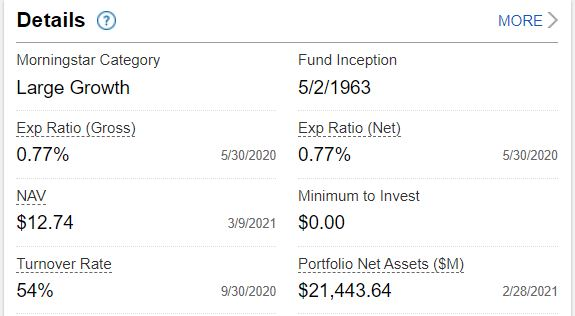
\includegraphics[width=\textwidth,keepaspectratio]{figures/slide13_img.JPG}
\caption{Fidelity Magellan Fund --- one of the best-known actively managed equity funds}
\end{figure}
\end{column}
\end{columns}
% Source slide 13 also had objective/strategy/risk screenshots (slide13_img1/2.JPG) -- dropped as redundant.
\end{frame}

% [src: 14, 15]
\begin{frame}{Types of Mutual Funds: Bond Funds}
\begin{itemize}
  \item Invest mainly in fixed-income securities
  \item Specific objective --- ``corporate,'' ``municipals'' --- relating to the types of bonds held
  \item Most also have a maturity objective relating to the average maturity of the portfolio's bonds
  \item Goal: outperform their benchmarks
\end{itemize}
\vspace{0.3em}
\begin{center}

\includegraphics[height=0.44\textheight,keepaspectratio]{figures/slide15_img_flat.png}
\end{center}
\begin{center}
\small United Asian High Yield Bond Fund
\end{center}
\end{frame}

% [src: 16]
\begin{frame}{Types of Mutual Funds: Four More Categories}
\begin{description}
  \item[Sector funds] Equity funds concentrating on a particular industry (e.g., Fidelity Select Health Care)
  \item[International funds] Invest in securities of firms located outside the United States
  \item[Balanced funds] Invest in both equities and bonds in relatively stable proportions
  \item[Asset allocation funds] May dramatically vary the proportions allocated to each asset according to the manager's forecast of relative performance
\end{description}
\end{frame}

% [src: 17, 18]
\begin{frame}{Growth of the Mutual Fund Industry}
\begin{columns}
\begin{column}{0.5\textwidth}
\centering
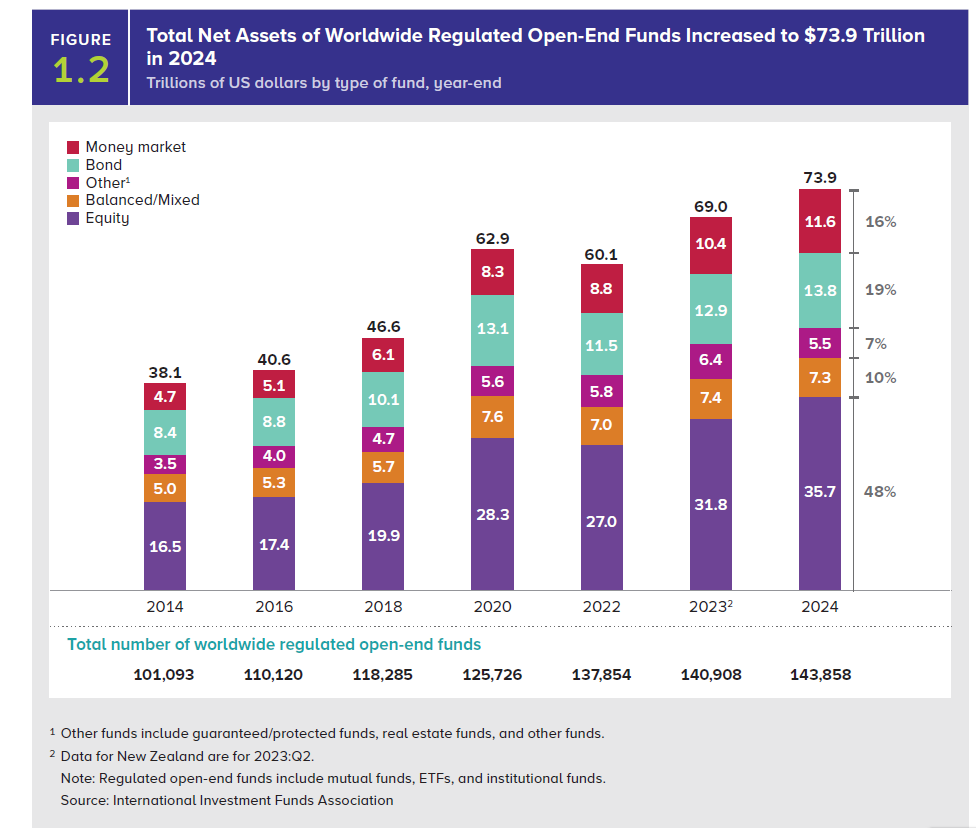
\includegraphics[width=\textwidth,keepaspectratio]{figures/slide17_img_flat.png}
\end{column}
\begin{column}{0.5\textwidth}
\centering

\includegraphics[width=\textwidth,keepaspectratio]{figures/slide18_img_flat.png}
\end{column}
\end{columns}
\vspace{0.2em}
\begin{center}
\small Source: 2025 Investment Company Factbook
\end{center}
\end{frame}

% [src: 19, 20]
\begin{frame}{Mutual Fund Returns: Three Ways to Earn}
\begin{description}
  \item[Income distribution] The fund earns dividends and interest on its portfolio securities and pays shareholders nearly all of this income (minus disclosed expenses) as dividends
  \item[Capital gains distribution] When the fund sells a security that has increased in price, it has a capital gain; at year-end most funds distribute these capital gains (minus capital losses) to investors
  \item[Increased NAV] If the market value of the portfolio increases after deduction of expenses and liabilities, the fund's NAV increases
\end{description}
% Source slide 20 (worked example) image was a corrupted/black screenshot -- dropped.
\note{For dividends and capital gains distributions, funds usually offer a choice: a check or other payment, or reinvestment in the fund to buy more shares (often without an additional sales load).}
\end{frame}

% [src: 21]
\begin{frame}{Costs of Investing: Fee Structure}
\begin{table}
\centering
\small
\begin{tabular}{p{0.19\textwidth}p{0.61\textwidth}p{0.1\textwidth}}
\toprule
\textbf{Fee} & \textbf{Definition} & \textbf{Timing} \\
\midrule
Operating expenses & Annual costs of operating the portfolio --- administrative expenses and advisory fees paid to the investment manager; range 0.5\%--1.25\% of total assets & Recurring \\
Front-end load & Commission or sales charge paid when purchasing shares; reduces the amount available to buy fund shares & One-time \\
Back-end load & ``Exit'' fee incurred when shares are redeemed; normally depends on the holding period and decreases to zero if held long enough & One-time \\
12b-1 fees & Annual fees charged to pay for marketing/distribution costs; limited to 1\% of a fund's average net assets & Recurring \\
\bottomrule
\end{tabular}
\end{table}
\note{12b-1 fees are annual charges assessed by certain mutual funds to cover distribution, marketing, and sometimes shareholder service costs. They are deducted directly from the fund's assets (reducing NAV and returns for all shareholders) and form part of the fund's overall expense ratio.}
\end{frame}

% [src: 22]
\begin{frame}{Fee Structures Vary Across Share Classes}
Mutual funds may offer different share classes representing ownership in the \emph{same} portfolio, but with different combinations of sales load and 12b-1 fees. An investor's \textbf{holding horizon} drives the choice between a higher front-end sales load and a higher 12b-1 fee.
\begin{center}

\includegraphics[height=0.55\textheight,keepaspectratio]{figures/slide22_img.png}
\end{center}
\begin{center}
\small Mishkin (2024), 13th edition --- fee schedule of the Dreyfus High Yield Fund share classes
\end{center}
\note{The 12b-1 is an ongoing ``load'' rather than a one-time upfront fee. Hence over longer holding periods an upfront load may be preferable to a 12b-1 fee. Some funds have back-end loads that are time-contingent and go away if you hold the shares long enough (typically about 5 years).}
\end{frame}

% [src: 23, 24]
\begin{frame}{Impact of Costs on Performance: Class A vs.\ Class C (4-Year Horizon)}
\textbf{Setup.} The Investments Fund sells Class A shares with a 6\% front-end load and no 12b-1 or back-end load fees; Class C shares carry 12b-1 fees of 0.5\% annually plus back-end load fees that start at 5\% and fall by 1\% for each full year held (until the 5th year). The portfolio's return net of operating expenses is 10\% annually. With \$1,000 to invest and a 4-year horizon:
\begin{itemize}
  \item \textbf{Class A:} invest \$940 net of load $\Rightarrow$ $\$940 \times (1+10\%)^{4} = \$1{,}376.25$
  \item \textbf{Class C:} invest the full \$1,000 at 9.5\% net of 12b-1 fees, then pay a 1\% back-end load: $\$1{,}000 \times (1+9.5\%)^{4} = \$1{,}437.66$, and $\$1{,}437.66 \times 0.99 = \$1{,}423.28$
\end{itemize}
\textbf{Class C is the better choice for a four-year horizon.}
\end{frame}

% [src: 25]
\begin{frame}{Impact of Costs on Performance: The 15-Year Horizon}
\textbf{Class A:} $\$940 \times (1+10\%)^{15} = \$3{,}926.61$
\vspace{0.4em}

\textbf{Class C:} no back-end load since the horizon exceeds five years, so $\$1{,}000 \times (1+9.5\%)^{15} = \$3{,}901.32$
\vspace{0.6em}

With a longer horizon, Class C is no longer better: the 0.5\% annual 12b-1 fee \emph{accumulates} over time and eventually overwhelms the one-time 6\% front-end load of Class A.
\end{frame}

% [src: 26, 27]
\begin{frame}{Index Funds}
\begin{itemize}
  \item Seek to \emph{replicate} (rather than beat) the performance of a benchmark index --- e.g., an S\&P 500 index fund closely tracks the S\&P 500
  \item Charge low fees: no equity research or stock selection to pay for
  \item Management cost is mainly fixed --- as assets grow, economies of scale allow further fee cuts, attracting more inflows
\end{itemize}
\vspace{0.2em}
\begin{center}
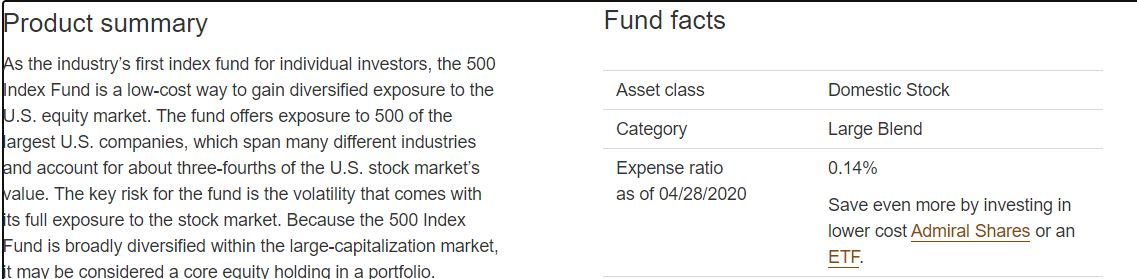
\includegraphics[width=0.62\textwidth,keepaspectratio]{figures/slide27_img.JPG}
\end{center}
\begin{center}
\small Vanguard 500 Index Fund
\end{center}
% Source slide 27 second screenshot (slide27_img1.JPG) dropped as redundant.
\note{The difference between the index fund return (row 1) and the S\&P 500 index return (row 2) is explained by the annual expense ratio.}
\end{frame}

% [src: 28]
\begin{frame}{Index Funds Charge Much Lower Fees Than Active Funds}
Average expense ratios of active funds have also declined over time --- mainly due to competition from index funds and ETFs.
\begin{center}

\includegraphics[height=0.62\textheight,keepaspectratio]{figures/slide28_img_flat.png}
\end{center}
\begin{center}
\small Source: 2025 Investment Company Factbook
\end{center}
\note{Expense ratios are measured as an asset-weighted average; the figure excludes mutual funds available as investment choices in variable annuities and funds that invest primarily in other mutual funds. The growing popularity of index funds has played a role in the overall decline in fund expense ratios.}
\end{frame}

% [src: 29]
\begin{frame}{Passive vs.\ Active Investing}
\begin{table}
\centering
\small
\begin{tabular}{p{0.12\textwidth}p{0.8\textwidth}}
\toprule
\textbf{Type} & \textbf{Objectives} \\
\midrule
Passive & Seek to \emph{match} the index benchmark. Hold securities for relatively long periods with infrequent changes. Markets are efficient --- switching among securities is useless. \\
Active & Seek to \emph{outperform} the index benchmark. Attempt to find mispriced stocks via fundamental or technical analysis. Some investors have comparative advantages in acquiring and analyzing information. \\
\bottomrule
\end{tabular}
\end{table}
% Source slide 29 image (slide29_img.jpg) dropped: decorative "ACTIVE/PASSIVE" signpost photo.
\end{frame}

% [src: 30, 31]
\begin{frame}{The Rise of Passive Investing}
\begin{columns}
\begin{column}{0.5\textwidth}
\centering
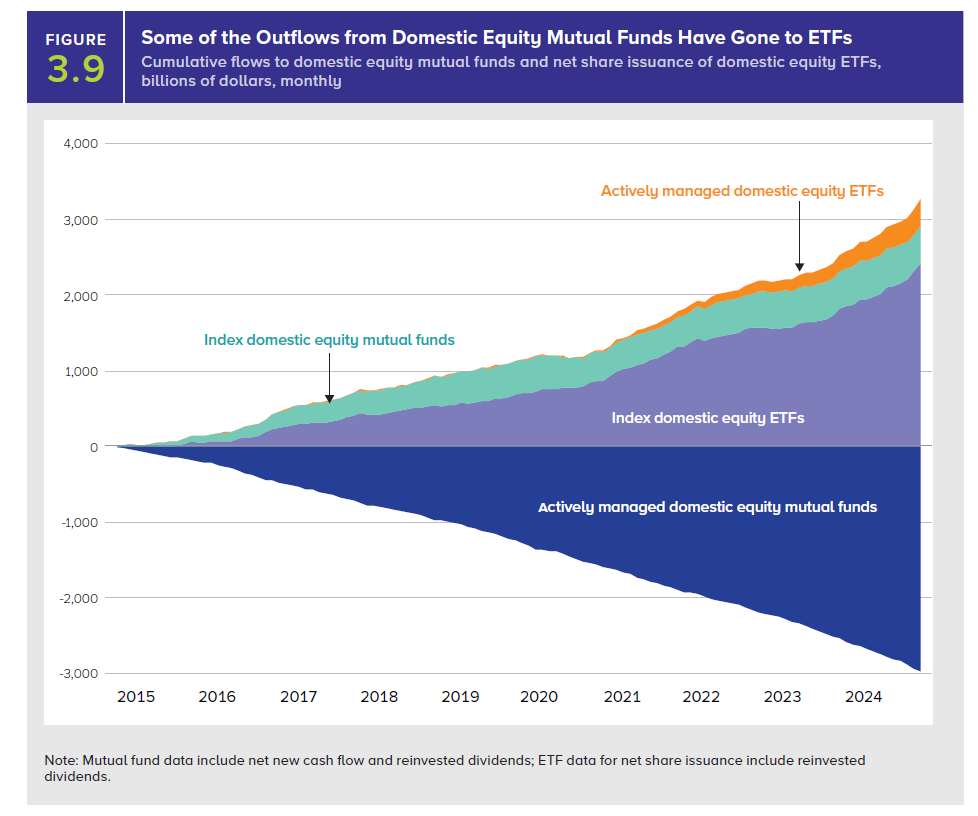
\includegraphics[width=\textwidth,keepaspectratio]{figures/slide30_img_flat.png}
\end{column}
\begin{column}{0.5\textwidth}
\centering
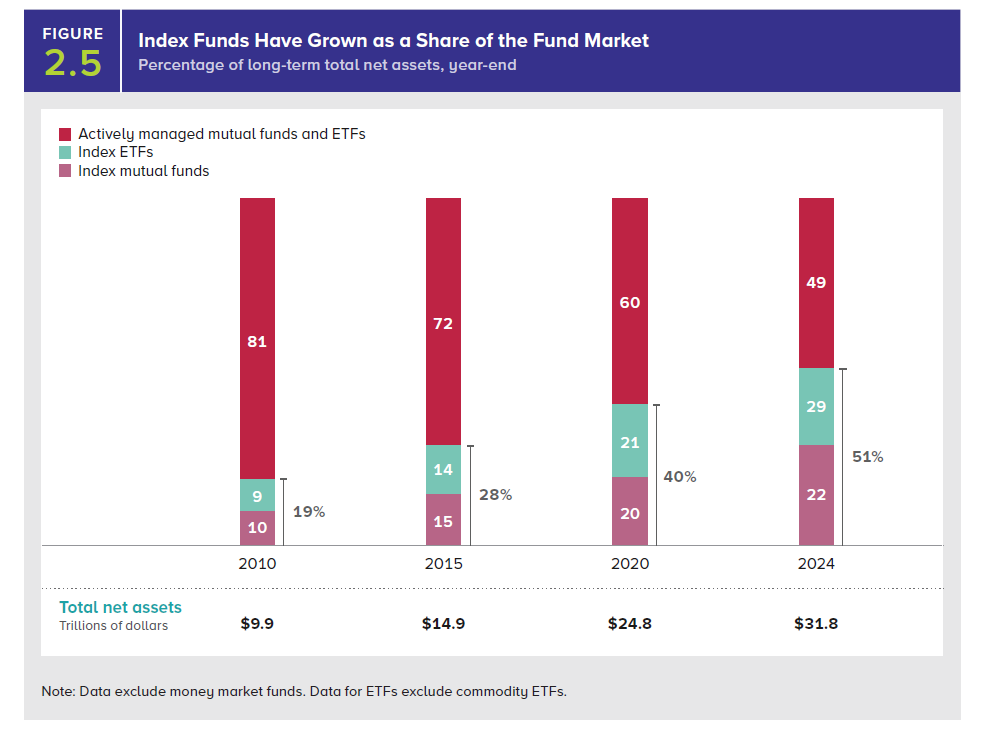
\includegraphics[width=\textwidth,keepaspectratio]{figures/slide31_img_flat.png}
\end{column}
\end{columns}
\vspace{0.2em}
\begin{center}
\small Source: 2025 Investment Company Factbook
\end{center}
\end{frame}

% [src: 32]
\begin{frame}{Buffett's Advice on Passive vs.\ Active}
In his 2013 letter to shareholders, Buffett disclosed the advice given to the trustee managing his cash bequest to his partner:
\begin{quote}
``My advice to the trustee could not be simpler: Put 10\% of the cash in short-term government bonds and 90\% in a very low-cost S\&P 500 index fund. (I suggest Vanguard's.) I believe the trust's long-term results from this policy will be superior to those attained by most investors --- whether pension funds, institutions or individuals --- who employ high-fee managers.''
\end{quote}
\note{Buffett on index funds: \href{https://www.youtube.com/watch?v=Z40yQoy9Nno}{youtube.com/watch?v=Z40yQoy9Nno}}
\end{frame}

% [src: 33, 34]
\begin{frame}{Closed-End Funds (CEFs)}
Created by issuing a \textbf{fixed number} of common shares to investors in an initial public offering. Once issued, shares are bought and sold by investors on stock exchanges and are \textbf{not} purchased from or redeemed by the fund; the assets are professionally managed per the fund's objectives and policies.
\vspace{0.3em}

The exchange price is set by demand and supply and may be greater or less than NAV:
\begin{center}

\includegraphics[height=0.45\textheight,keepaspectratio]{figures/slide34_img_flat.png}
\end{center}
\begin{center}
\small Source: 2025 Investment Company Factbook
\end{center}
\note{Closed-end funds most of the time trade at a price discount relative to their NAV.}
\end{frame}

% [src: 35]
\begin{frame}{Total Assets of Closed-End Funds}
\begin{figure}
\centering

\includegraphics[height=0.72\textheight,keepaspectratio]{figures/slide35_img_flat.png}
\end{figure}
\begin{center}
\small Source: 2025 Investment Company Factbook
\end{center}
\end{frame}

% [src: 36, 38]
\begin{frame}{Exchange-Traded Funds (ETFs)}
Like index funds, ETFs are generally designed to track a particular index (e.g., S\&P 500) --- but they trade on stock exchanges throughout the day and are highly liquid.
\vspace{0.3em}

\textbf{Uses:} long-term asset allocation (advisors build diversified portfolios); intermediate-term sector rotation / tactical allocation (low-cost access to countries, sectors, assets); short-term speculation (quick position changes, short selling, leveraged positions).
\vspace{0.3em}

\textbf{ETFs vs.\ index funds:}
\begin{itemize}
  \item ETF shares trade on exchanges \emph{intraday}, via brokers (commissions apply); redeemable from the fund itself only in very large blocks
  \item ETF price may differ from NAV: price reflects secondary-market demand/supply, NAV reflects the market value of underlying assets --- \textbf{arbitrage keeps the two close}
\end{itemize}
\note{An ETF is a type of investment company (open-end or UIT) whose objective is to achieve the same return as a particular market index. Pursuant to SEC exemptive orders, ETF shares trade on a secondary market and are only redeemable from the fund itself in very large blocks.}
\end{frame}

% [src: 37]
\begin{frame}{Growth of ETFs}
\begin{figure}
\centering

\includegraphics[height=0.72\textheight,keepaspectratio]{figures/slide37_img_flat.png}
\end{figure}
\begin{center}
\small Source: 2025 Investment Company Factbook
\end{center}
\end{frame}

% [src: 39]
\begin{frame}{Creation/Redemption of ETF Shares}
\begin{figure}
\centering

\includegraphics[height=0.72\textheight,keepaspectratio]{figures/slide39_img.png}
\end{figure}
\begin{center}
\small Source: ICI 2026 Investment Company Fact Book (released April 27, 2026; 2025 data)
\end{center}
\end{frame}

% [src: 40]
\begin{frame}{Comparing Different Types of Funds}
\begin{table}
\centering
\small
\begin{tabular}{p{0.06\textwidth}p{0.275\textwidth}p{0.275\textwidth}p{0.275\textwidth}}
\toprule
 & \textbf{Closed-End Funds} & \textbf{Open-End Funds} & \textbf{Index Funds} \\
\midrule
Pros & Traded on exchange; can buy and sell any time the market is open & Fund size is unlimited; price = NAV & Passive investing; lower fees; lower turnover \\
Cons & Fund size is fixed; share price can deviate from NAV & Not listed on exchange; only one price (NAV) per day, after the market closes & Not listed on exchange; only one price (NAV) per day \\
\bottomrule
\end{tabular}
\end{table}
\end{frame}

% [src: 41]
\section{Hedge Funds}
% Source slide 41 image (slide41_img.jpg) dropped: decorative photo.

% [src: 42]
\begin{frame}{What Is a Hedge Fund?}
A \textbf{partnership} where investors pool money and a fund manager deploys it across a variety of assets using sophisticated investment techniques.
\begin{itemize}
  \item Accessible only to accredited and/or institutional investors
  \item Can use leverage, take short positions, and hold long/short derivative positions
  \item Less strictly regulated by the SEC than mutual funds
\end{itemize}
\vspace{0.3em}
Hedge funds seek \textbf{absolute returns} --- exploiting opportunities while protecting principal --- materially different from the mutual-fund manager, who is tied to an index benchmark.
\note{Source: AIMA's Roadmap to Hedge Funds, \href{http://www.aima.org/en/knowledge_centre/education/aimas-roadmap-to-hedge-funds.cfm}{aima.org}.}
\end{frame}

% [src: 43]
\begin{frame}{Key Features of Hedge Funds}
\begin{description}
  \item[Organizational structure] Private partnership in the U.S.: limited partners (investors) vs.\ general partners (fund manager)
  \item[Fee structure] ``2/20'': management fee of 2\% of assets + performance fee of 20\% of profits
  \item[Liquidity] Initial 1--5 year lockup period with no redemptions; after lockup, some funds limit redemptions to once a quarter, and most require 15--90 days advance notice
\end{description}
\note{Redemptions are restricted by lockup periods and required notices well before the redemption. Hedge funds restrict redemptions so the manager is not forced to sell or close out positions at bad prices simply because investors are panicking. Sometimes funds can borrow to pay for redemptions, but if there are too many at once this breaks down.}
\end{frame}

% [src: 44, 45, 46]
\begin{frame}{Hedge Funds vs.\ Mutual Funds}
\begin{table}
\centering
\small
\begin{tabular}{p{0.15\textwidth}p{0.37\textwidth}p{0.37\textwidth}}
\toprule
 & \textbf{Hedge Fund} & \textbf{Mutual Fund} \\
\midrule
Transparency & Minimal disclosure of strategy and portfolio composition & Regulation requires public disclosure of strategy and portfolio composition \\
Investors & No more than 100 ``sophisticated'' and wealthy investors & Number not limited \\
Strategies & Very flexible and opportunistic; wide range of assets; often shorting, leverage, and derivatives & Predictable, stable strategies stated in prospectus; limited shorting, leverage, derivatives \\
Liquidity & Lock-up periods; advance redemption notices & Purchase or redeem shares daily \\
Compensation & Management fee 1--2\% of assets + performance fee 15--20\% of profits & Usually a fixed percentage of assets, typically 0.5\%--1.25\% \\
\bottomrule
\end{tabular}
\end{table}
\note{See the example of Bill Ackman during the 2020 COVID-19 crash: \href{https://www.barrons.com/articles/the-greatest-trade-of-all-timeand-what-bill-ackman-is-investing-in-now-51600457809}{barrons.com --- ``The Greatest Trade of All Time''}.}
\end{frame}

% [src: 47]
\begin{frame}{Assets Under Management by Hedge Funds}
Global hedge fund AUM has grown substantially over the past decades, with notable dips around the 2008 global financial crisis and the 2020 COVID drawdown, before reaching a record \$4.54 trillion at end-2025 (HFR), with net inflows above \$300 billion --- Preqin projects \$4.8--5.0 trillion by end-2026.
\begin{center}

\includegraphics[height=0.50\textheight,keepaspectratio]{figures/slide47_img_flat.png}
\end{center}
\begin{center}
\small Source: HFR (Q4 2025); Preqin projections
\end{center}
\end{frame}

% [src: 48]
\begin{frame}{Hedge Fund Strategies}
\begin{figure}
\centering
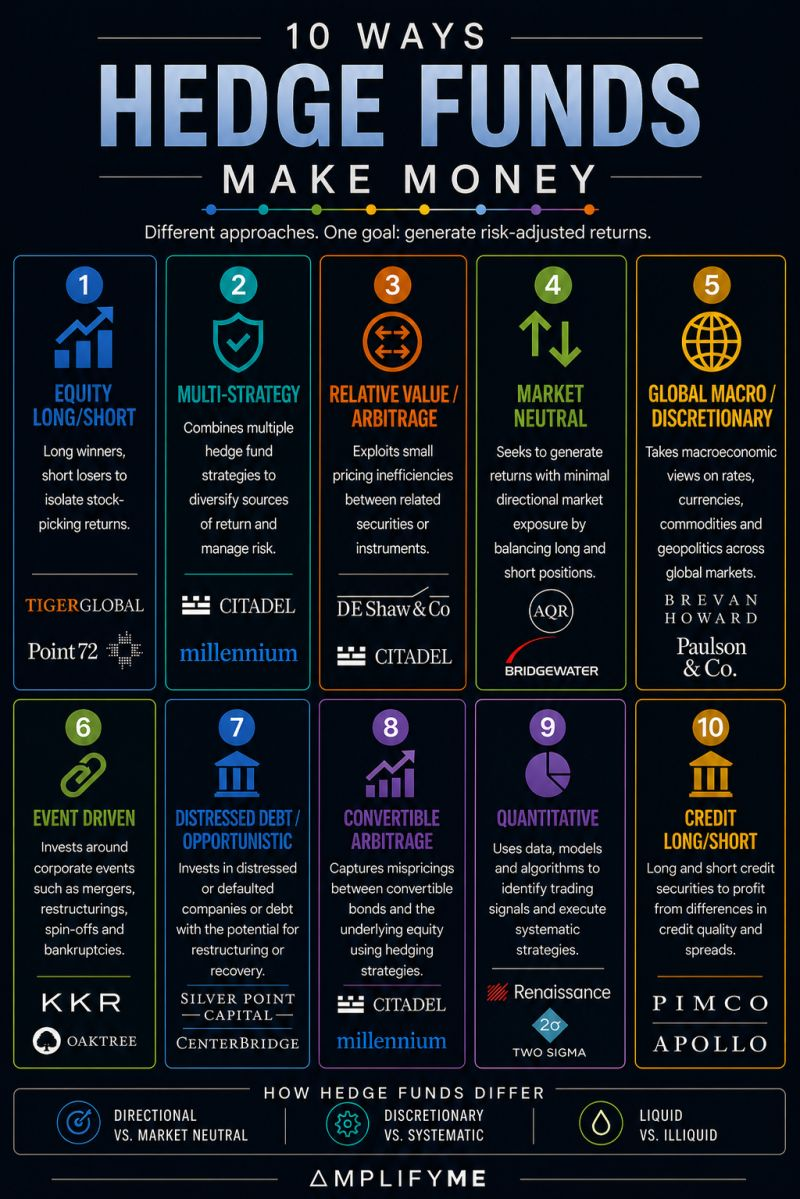
\includegraphics[height=0.70\textheight,keepaspectratio]{figures/slide48_img.jpg}
\end{figure}
\end{frame}

% [src: 49]
\begin{frame}{Hedge Fund Strategies: Equity Hedge and Event-Driven}
\textbf{Equity hedge} --- combine long positions in expected outperformers with short positions in expected underperformers, net market exposure varying with manager conviction and risk assessment.
\begin{itemize}
  \item Two alpha sources: security selection on both the long and short sides
  \item Leverage: gross exposure typically 150\%--300\% to amplify stock-specific returns
\end{itemize}
\vspace{0.3em}
\textbf{Event-driven} --- exploit price movements surrounding corporate events.
\vspace{0.2em}
\begin{center}

\includegraphics[height=0.42\textheight,keepaspectratio]{figures/slide49_img_flat.png}
\end{center}
\end{frame}

% [src: 50]
\begin{frame}{Hedge Fund Strategies: The Remaining Families}
\begin{description}
  \item[Relative value arbitrage] Seek to profit from pricing discrepancies between related securities, with neutral or limited market exposure
  \item[Macro \& systematic] Discretionary vs.\ systematic implementation
  \item[Multi-strategy platforms] Autonomous investment teams with defined risk budgets within centralized oversight
\end{description}
\vspace{0.2em}
\begin{center}

\includegraphics[width=0.7\textwidth,keepaspectratio]{figures/slide50_img_flat.png}
\end{center}
\end{frame}

% [src: 51]
\begin{frame}{Strategy-Based AUM Breakdown}
\begin{figure}
\centering

\includegraphics[height=0.72\textheight,keepaspectratio]{figures/slide51_img_flat.png}
\end{figure}
\end{frame}

% [src: 52]
\begin{frame}{Who Are the Investors?}
\begin{itemize}
  \item Originally: primarily high-net-worth individuals (HNWI) and family offices
  \item Over time institutional investors grew --- the post-GFC search for yield pushed money in
  \item Recently the trend reversed: private capital (family offices, HNWI) is again the largest source of hedge fund capital
\end{itemize}
\vspace{0.2em}
\begin{columns}
\begin{column}{0.5\textwidth}
\centering

\includegraphics[width=\textwidth,keepaspectratio]{figures/slide52_img.png}
\end{column}
\begin{column}{0.5\textwidth}
\centering

\includegraphics[width=\textwidth,keepaspectratio]{figures/slide52_img1.png}
\end{column}
\end{columns}
\end{frame}

% [src: 53]
\begin{frame}{Fee Structure in Hedge Funds}
\begin{description}
  \item[Management fees] Computed as a percent of assets under management; run between 1\% and 2\%
  \item[Performance (incentive) fees] A share of positive returns earned above a benchmark; the average is 20\%, but varies substantially (Steve Cohen's SAC Capital charged 50\%)
  \item[Hurdle rate] A benchmark return that must be realized before a performance fee can be assessed
  \item[High-water mark] No performance fee unless the fund's NAV exceeds the highest NAV previously recorded
\end{description}
\end{frame}

% [src: 54, 55]
\begin{frame}{High-Water Mark}
\begin{columns}
\begin{column}{0.52\textwidth}
\begin{figure}
\centering
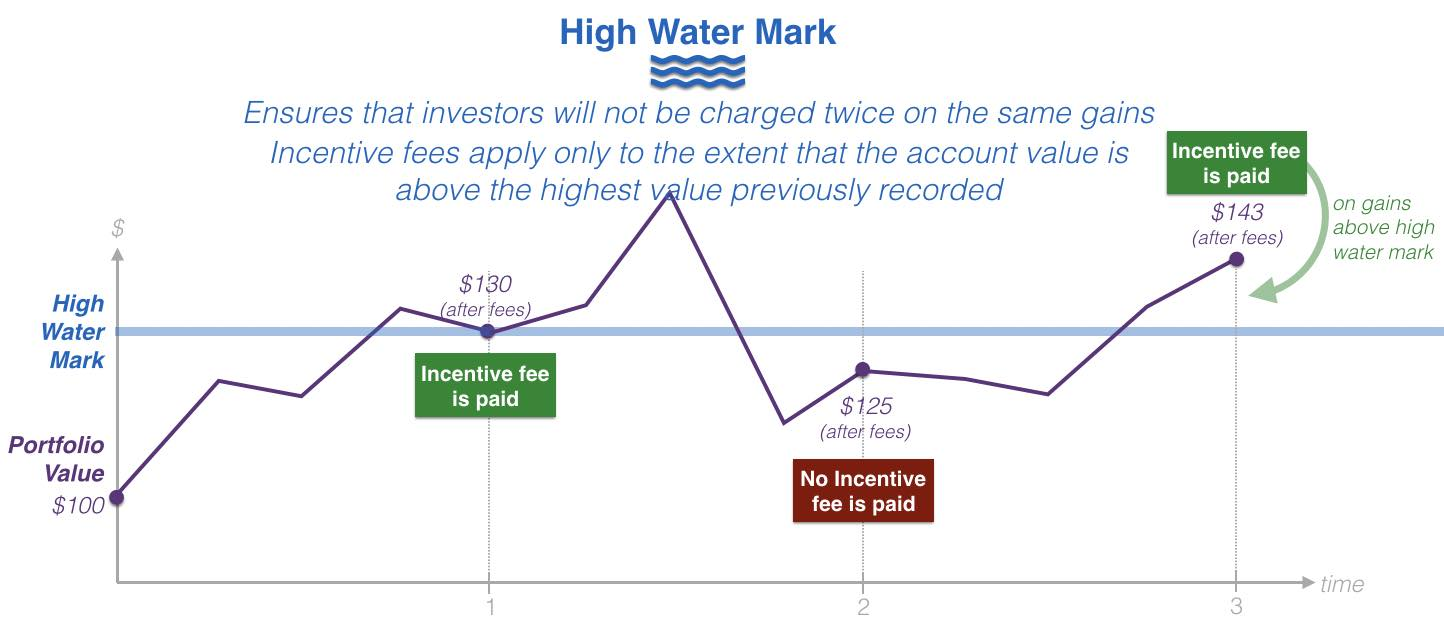
\includegraphics[width=\textwidth,keepaspectratio]{figures/slide54_img.jpg}
\end{figure}
\end{column}
\begin{column}{0.46\textwidth}
The NAV increase from 125 to 130 in year 3 merely recovers a previous loss --- only the increase from 130 to 143 is charged an incentive fee.
\vspace{0.4em}

High-water marks can give managers an incentive to \textbf{shut down} a poorly performing fund: with deep losses, recovering the previous peak may be too difficult. This may explain the high failure rate of hedge funds --- about 22\% of funds operating in a year closed over the next three years (Morningstar).
\end{column}
\end{columns}
\end{frame}

% [src: 56, 57]
\begin{frame}{Hedge Fund Fee Structure: Example}
A hedge fund has \$1 million AUM, a ``2 and 20'' fee structure, and a 5\% hurdle rate. Gross return this year: 20\%. Performance fees are calculated on \emph{gross} returns (not net of management fees).
\begin{itemize}
  \item Management fee: $\$1{,}000{,}000 \times 2\% = \$20{,}000$
  \item Dollar return above the hurdle: $\$1{,}000{,}000 \times (20\%-5\%) = \$150{,}000$ --- the base against which incentive fees are charged
  \item Performance fee: $\$150{,}000 \times 20\% = \$30{,}000$
\end{itemize}
\textbf{Total fees paid to the manager: \$20{,}000 + \$30{,}000 = \$50{,}000.}
\end{frame}

% [src: 58]
\begin{frame}{Hedge Fund Fee Structure}
\begin{figure}
\centering

\includegraphics[height=0.62\textheight,keepaspectratio]{figures/slide58_img.png}
\end{figure}
\begin{center}
\small Source: KPMG, \emph{Generation Alpha: The Hedge Fund Industry Landscape and Outlook for 2026}; Morgan Stanley, \emph{Hedge Funds 2026 Outlook}
\end{center}
\note{Morgan Stanley's \emph{Hedge Funds 2026 Outlook} themes: (1) AI and ``platformification'' of the investment process moving from experimental to essential; (2) fee compression alongside the dominance of multi-strategy platforms (Millennium, Citadel, Balyasny).}
\end{frame}

% [src: 59]
\begin{frame}{Hedge Fund Performance vs.\ S\&P 500}
\begin{figure}
\centering

\includegraphics[height=0.68\textheight,keepaspectratio]{figures/slide59_img_flat.png}
\end{figure}
\begin{center}
\small Source: Hedge Fund Research. Values indexed to 100 at end-1989 (cumulative growth of \$100 invested at the start of 1990).
\end{center}
\note{Index descriptions: \href{https://www.hedgefundresearch.com/hfri-indices-index-descriptions}{hedgefundresearch.com --- HFRI index descriptions}.}
\end{frame}

% [src: 60]
\begin{frame}{Hedge Fund Performance: What the 36 Years Show}
\begin{itemize}
  \item \textbf{Long-term underperformance:} S\&P 500 grew 100 $\to$ 4,011 (3,911\% cumulative) vs.\ hedge funds 100 $\to$ 2,335 (2,235\%)
  \item \textbf{Lower volatility, downside protection:} 2008 crisis --- HFRI $-19\%$ vs.\ S\&P 500 $-37\%$; 2002 dot-com bust --- HFRI $-1.45\%$ vs.\ S\&P 500 $-22.1\%$; in the volatile Q1 2026 (VIX above 50), HFRI $+0.36\%$ vs.\ S\&P 500 total return $-4.33\%$
  \item \textbf{Divergence periods:} comparable through the 1990s--early 2000s; S\&P 500 pulled away dramatically post-2009 and kept widening the gap over 2015--2026 despite positive HF returns in most years (YTD 2026 through July: HFRI $+6.25\%$ vs.\ S\&P 500 $+10.1\%$)
  \item \textbf{Risk-adjusted view:} lower volatility may have delivered better risk-adjusted returns in turbulent periods --- relevant for investors prioritizing capital preservation
\end{itemize}
\end{frame}

% [src: 61]
\begin{frame}{Hedge Fund Performance Decomposition}
\begin{figure}
\centering
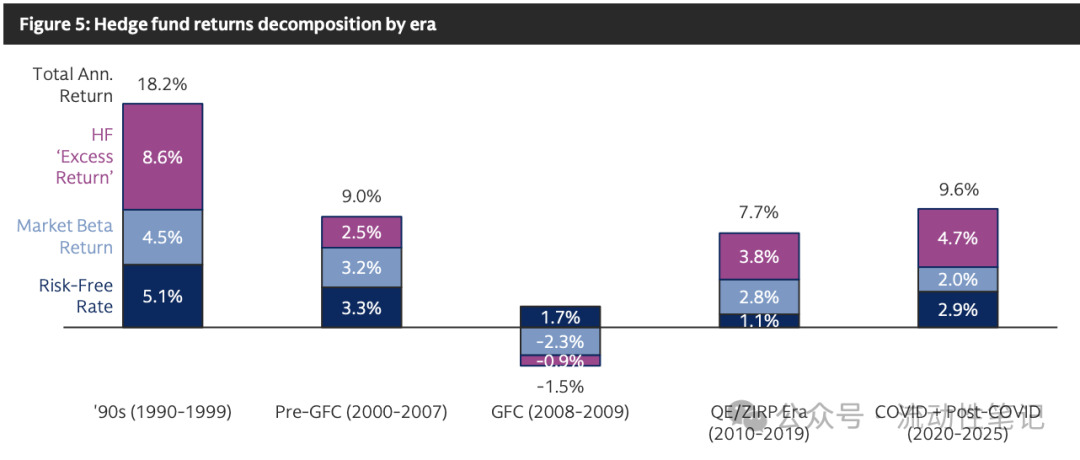
\includegraphics[height=0.62\textheight,keepaspectratio]{figures/slide61_img.jpg}
\end{figure}
\begin{center}
\small Source: KPMG, \emph{Generation Alpha: The Hedge Fund Industry Landscape and Outlook for 2026}; Morgan Stanley, \emph{Hedge Funds 2026 Outlook}
\end{center}
\end{frame}

% [src: 62, 63]
\begin{frame}{Warren Buffett's Hedge Fund Bet}
\begin{columns}
\begin{column}{0.48\textwidth}
\centering
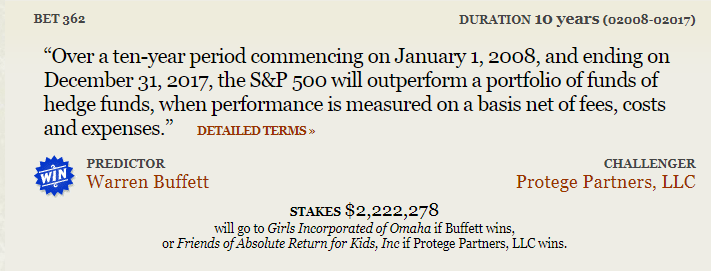
\includegraphics[width=\textwidth,keepaspectratio]{figures/slide62_img.png}
\end{column}
\begin{column}{0.48\textwidth}
\centering
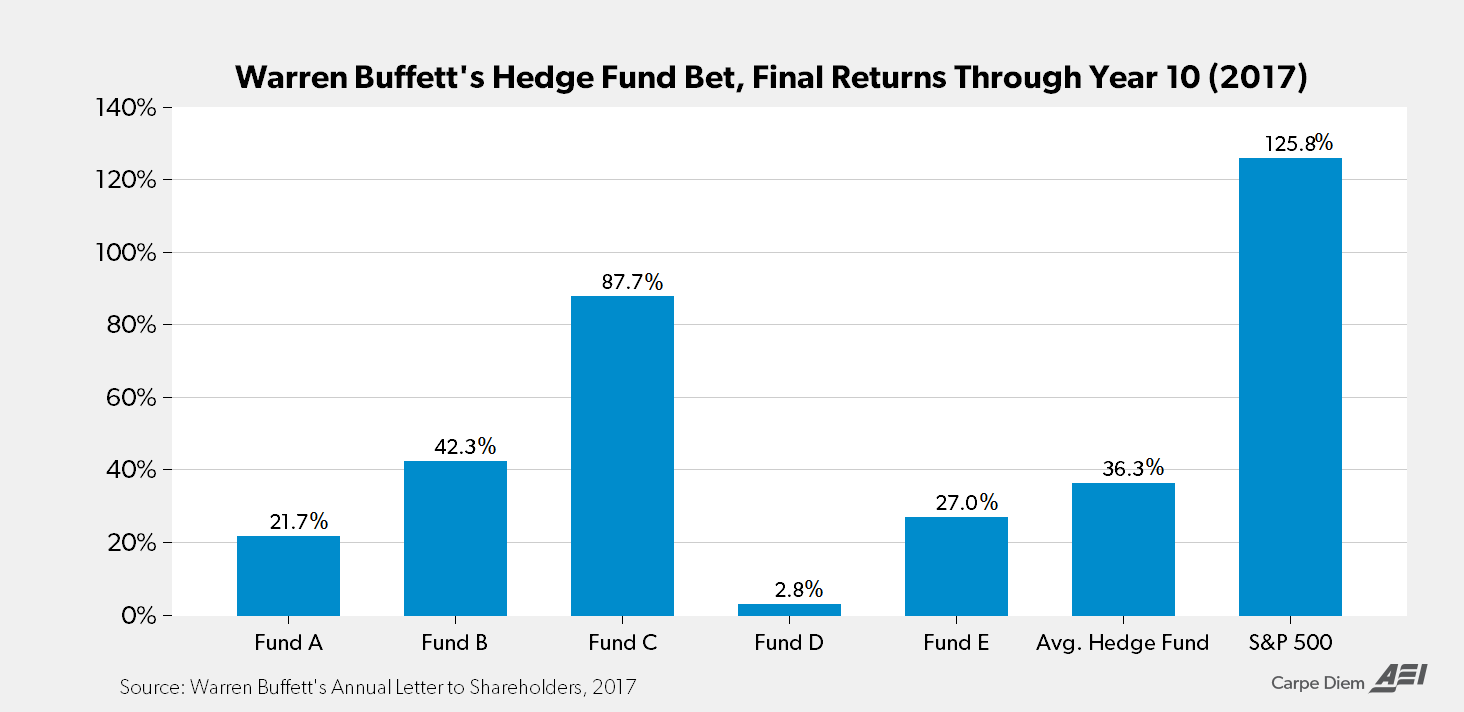
\includegraphics[width=\textwidth,keepaspectratio]{figures/slide63_img.png}
\end{column}
\end{columns}
\vspace{0.2em}
\begin{center}
\small Source: \href{http://longbets.org/362/\#adjudication_terms}{longbets.org/362}
\end{center}
% Source slide 62 extra images (slide62_img1.png, slide62_img.jpg) dropped: duplicate/bettor photos.
\end{frame}

% [src: 64, 65]
\begin{frame}{Funds of Funds (FoFs) and Their Fees}
\textbf{FoFs} are investment companies that invest in multiple hedge funds. They often have lower minimum investment thresholds than traditional hedge funds and can sell shares to a larger number of investors; they are supposed to provide due diligence in screening hedge funds for investment worthiness.
\vspace{0.3em}

\textbf{But:} you pay \emph{two layers} of fees --- to the FoF and to each underlying hedge fund.
\begin{itemize}
  \item The FoF pays an incentive fee to each underlying fund that beats its hurdle, \emph{even if} aggregate performance is poor --- diversification can hurt the investor here
  \item If the underlying funds use similar strategies, diversification may be an illusion
\end{itemize}
\end{frame}

% [src: 66]
\begin{frame}{Incentive Fees in Funds of Funds: Example}
A FoF invests \$1 million in each of three hedge funds. Hurdle rate: zero return. Each fund charges a 20\% incentive fee. Gross return of the FoF: $-5\%$.
\begin{itemize}
  \item Any underlying fund with a positive return still collects its incentive fee
  \item The FoF \textbf{still pays incentive fees of \$0.12 for every \$3 invested}, despite losing money overall
\end{itemize}
\vspace{0.2em}
\begin{center}
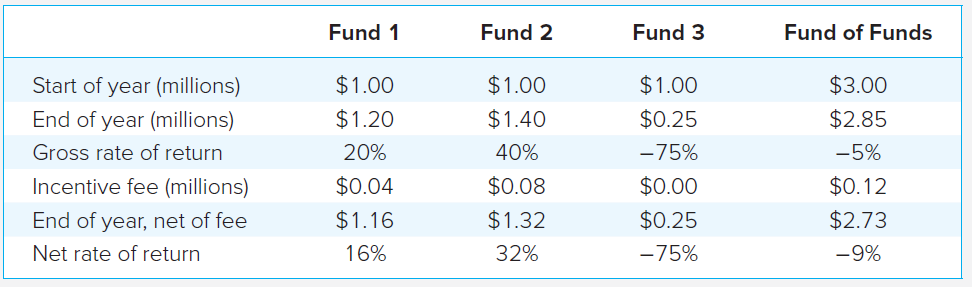
\includegraphics[height=0.44\textheight,keepaspectratio]{figures/slide66_img.png}
\end{center}
\end{frame}

% [src: 67, 68]
\begin{frame}{Key Takeaways}
\begin{description}
  \item[Investment companies] Pool investor funds for diversification, professional management, and low minimums; priced at NAV
  \item[Mutual funds (open-end)] Money market, equity, bond, sector, international types; returns via income distributions, capital gains distributions, NAV appreciation; front/back-end loads, 12b-1 fees, expense ratios --- fees significantly impact long-term returns; passive investing is rising globally
  \item[Closed-end funds] Fixed shares, traded on exchanges at a premium or discount to NAV
  \item[ETFs] Index-fund features plus intraday trading; the creation/redemption arbitrage mechanism keeps price close to NAV; low-cost, flexible tools for allocation, rotation, or speculation
  \item[Hedge funds] Private partnerships for accredited investors; leverage, shorting, derivatives; absolute-return objective; ``2 and 20'' with high-water mark; lower volatility and downside protection vs.\ S\&P 500, but long-term absolute underperformance
  \item[Funds of funds] Diversification across hedge funds, but two layers of fees
\end{description}
\end{frame}

\end{document}
